\documentclass[12pt, a4paper]{report}

\usepackage[czech]{babel}
\usepackage[IL2]{fontenc}
\usepackage[utf8]{inputenc}
\usepackage{lmodern}  % lepší kvalita PDF

\usepackage[a4paper,top=3cm,bottom=3cm,left=3cm,right=3cm,marginparwidth=1.75cm]{geometry}

\usepackage{amsmath}
\usepackage{graphicx}
\usepackage{titling}
\usepackage{enumitem}
\usepackage[colorlinks=true, allcolors=black]{hyperref}
\usepackage{url}
\usepackage{caption}
\usepackage{float}

\usepackage{pdfpages}


% formátování zdrojového kódu
\usepackage{listings}
\usepackage{color}

\definecolor{dkgreen}{rgb}{0,0.6,0}
\definecolor{gray}{rgb}{0.5,0.5,0.5}
\definecolor{mauve}{rgb}{0.58,0,0.82}

\lstset{frame=tb,
	language=C,
	aboveskip=3mm,
	belowskip=3mm,
	showstringspaces=false,
	columns=flexible,
	basicstyle={\small\ttfamily},
	numbers=none,
	numberstyle=\tiny\color{gray},
	keywordstyle=\color{blue},
	commentstyle=\color{dkgreen},
	stringstyle=\color{mauve},
	breaklines=true,
	breakatwhitespace=true,
	tabsize=4,
	extendedchars=true,
	literate=%
	{á}{{\'a}}1
	{č}{{\v{c}}}1
	{ď}{{\v{d}}}1
	{é}{{\'e}}1
	{ě}{{\v{e}}}1
	{í}{{\'i}}1
	{ň}{{\v{n}}}1
	{ó}{{\'o}}1
	{ř}{{\v{r}}}1
	{š}{{\v{s}}}1
	{ť}{{\v{t}}}1
	{ú}{{\'u}}1
	{ů}{{\r{u}}}1
	{ý}{{\'y}}1
	{ž}{{\v{z}}}1
	{Á}{{\'A}}1
	{Č}{{\v{C}}}1
	{Ď}{{\v{D}}}1
	{É}{{\'E}}1
	{Ě}{{\v{E}}}1
	{Í}{{\'I}}1
	{Ň}{{\v{N}}}1
	{Ó}{{\'O}}1
	{Ř}{{\v{R}}}1
	{Š}{{\v{S}}}1
	{Ť}{{\v{T}}}1
	{Ú}{{\'U}}1
	{Ů}{{\r{U}}}1
	{Ý}{{\'Y}}1
	{Ž}{{\v{Z}}}1
}
\lstset{language=C}


% údaje na titulní straně
\title{Online puzzle}
\def \thesubtitle {Semestrální práce z předmětu KIV/UPS}
\author{Patrik Harag}
\def \theauthoremail {harag@students.zcu.cz}
\def \theauthorid {(A15B0034P)}

\begin{document}

\begin{titlepage}
	\begin{figure}
		
\includegraphics[height=50mm]{img-fav-logo}
	\end{figure}
	
	\centering
	{\large \hspace{1mm} \par} % tady musí být nějaký text jinak nefunguje vertikální odsazení
	\vspace{15ex}
	
	{\scshape\Large \thesubtitle \par}
	\vspace{1.5ex}
	{\huge\bfseries \thetitle \par}
	\vspace{2ex}
	{\Large\itshape \theauthor \par}
	\vspace{2ex}
	{\texttt{\theauthoremail} \par}
	\vspace{1ex}
	{\texttt{\theauthorid} \par}
	\vspace{5ex}
	%{{Celková doba řešení: \textgreaterX h} \par}
	
	\vfill

	{\large \today\par}
\end{titlepage}

% strana s obsahem
\setcounter{page}{0} 
\tableofcontents
\thispagestyle{empty}


\chapter{Úvod}
\section{Zadání}
Online puzzle, kde hráči společnými silami skládají puzzle. Dílky bude možné volně přesouvat po herní ploše, a to jednotlivě i po skupinách. Bude zahrnovat server v jazyce C a klienta v Javě.

\section{Zásady vypracování}
\begin{itemize}
	\item Úlohu naprogramujte v programovacím jazyku C/C++ anebo Java. Pokud se jedná o úlohu server/klient, pak klient bude v Javě a server v C/C++.
	\item Komunikace bude realizována textovým nešifrovaným protokolem nad TCP protokolem.
	\item Výstupy serveru budou v alfanumerické podobě, klient může komunikovat i v grafice (není podmínkou).
	\item Server řešte pod operačním systémem Linux, klient může běžet pod OS Windows XP. Emulátory typu Cygwin nebudou podporovány.
	\item Realizujte konkurentní (paralelní) servery. Server musí být schopen obsluhovat požadavky více klientů souběžně.
	\item Součástí programu bude trasování komunikace, dovolující zachytit proces komunikace na úrovni aplikačního protokolu a zápis trasování do souboru.
	\item Každý program bude doplněn o zpracování statistických údajů (přenesený počet bytů, přenesený počet zpráv, počet navázaných spojení, počet přenosů zrušených pro chybu, doba běhu apod.).
	\item Zdrojové kódy organizujte tak, aby od sebe byly odděleny části volání komunikačních funkcí, které jste vytvořili na základě zadání, od částí určených k demonstraci funkčnosti vašeho řešení (grafické rozhraní).
\end{itemize}

\chapter{Programátorská dokumentace}
\section{Server}

\paragraph{Použité nástroje}
 Server byl vyvinut v C 99.

\paragraph{Základní návrh}
Program pracuje ve dvou vláknech. Hlavní vlákno po inicializaci prostředí přijímá nová spojení. Druhé vlákno obsluhuje klienty a vyhodnocuje stav her. Toto řešení se ukázalo jako nejlepší z následujících důvodů:
\begin{itemize}
	\item jednoduchost -- v podstatě celá herní logika v jednom vlákně,
	\item na straně serveru se neprovádí žádné výpočetně náročné operace,
	\item cílový server stejně nebude mít více fyzických procesorových jader (VPS).
\end{itemize}
Když hlavní vlákno přijme spojení, vytvoří novou \emph{session} (více o \emph{session} viz dále) a čeká na další spojení. Druhé vlákno postupně prochází všechny \emph{session} a reaguje na jejich zprávy. Každý socket je nastaven jako neblokující.

\paragraph{Ukládání a načítání}
Je prováděno automaticky při startu a ukončení programu. Jako formát pro uložení je využit samotný síťový protokol. Načtení je realizováno formou simulace spojení. To znamená, že serveru je předána série zpráv, které zpracuje stejným způsobem jako při běžném chodu a tím uvede server do požadovaného stavu.

\paragraph{Testy}
Server je testován integračními testy s využitím klientského API.

\subsection{Seznam zdrojových souborů}
\begin{itemize}
	\item \emph{main.c} -- obsahuje vstupní funkci, zpracovává parametry a spouští server.
	\item \emph{buffer.c/h} -- pomocná struktura používaná hlavně pro dočasné ukládání zpráv (po přijetí, před odesláním).
	\item \emph{utils.c/h} -- obsahuje různé pomocné funkce.
	\item \emph{server.c/h} -- obsahuje základní logiku serveru.
	\item \emph{session.c/h} -- obsahuje strukturu pro ukládání dat o jednom spojení + funkce které s nimi pracují.
	\item \emph{session\_pool.c/h} -- spravuje všechny \emph{session} na jednom místě.
	\item \emph{game.c/h} -- obsahuje strukturu pro ukládání dat o jedné hře + funkce které s nimi pracují.
	\item \emph{game\_pool.c/h} -- spravuje všechny \emph{game} na jednom místě.
	\item \emph{shared.c/h} -- spravuje sdílený herní stav, zastřešuje \emph{session\_pool} a \emph{game\_pool}. Ukládá a načítá herní stav do souboru.
	\item \emph{controller.c/h} -- zpracovává přijaté zprávy.
	\item \emph{protocol.h} -- obsahuje konstanty síťového protokolu.
	\item \emph{stats.c/h} -- spravuje statistiky.
\end{itemize}

\subsection{Důležité datové struktury}

\subsubsection*{Session}
Tato datová struktura, která se nachází v souboru \emph{session.h}, ukládá informace o jednom spojení. Může představovat i hráče, ovšem po přerušení spojení a následovném opětovném navázání bude vytvořena zcela nová instance.

Přístup k instancím této struktury musí být řízen, jelikož k nim přistupují obě vlákna.

\begin{lstlisting}
typedef struct _Session {

	int id;
	SessionStatus status;
	
	int socket_fd;
	unsigned long long last_activity;
	unsigned long long last_ping;
	Buffer to_send;
	int corrupted_messages;
	
	char name[SESSION_PLAYER_MAX_NAME_LENGTH + 1];
	Game* game;

} Session;
\end{lstlisting}

\subsubsection*{Game}
Struktura ze souboru \emph{game.h}, která obsahuje stav jedné hry.

\begin{lstlisting}
typedef struct _Game {
	int id;
	unsigned int w, h;
	Piece** pieces;
	bool finished;
} Game;

typedef struct _Piece {
	int id;
	int x, y;
} Piece;
\end{lstlisting}

\newpage

\section{Klient}
Klient je realizován v programovacím jazyce Java 8. Pro uživatelské rozhraní a je použit framework JavaFX.


\subsection{Balíček cz.harag.puzzle.app}
Obsahuje aplikační část -- vstupní třídu, která zpracovává vstup z příkazové řádky a grafické uživatelské rozhraní.

Důležitou úlohu zde hraje rozhraní \emph{Page}, které představuje jednu stránku. Existuje například stránka pro přihlášení, vytvoření hry, stránka s chybou atd.

\begin{figure}[H]
	\centering
	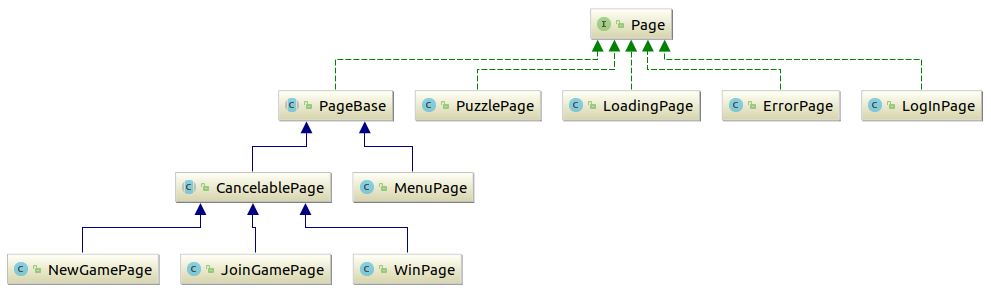
\includegraphics[width=1\linewidth]{img-page-h}
	\caption{Diagram tříd -- rozhraní \emph{Page}.}
	\label{fig:img-page-h}
\end{figure}

\subsection{Balíček cz.harag.puzzle.net}
Obsahuje síťovou část.

\paragraph{Třídy:}
\begin{itemize}
	\item \emph{Connection} -- zprostředkuje posílání a příjímání zpráv.
	\item \emph{ConnectionHolder} -- obaluje \emph{Connection}, poskytuje vyšší abstrakci, udržuje spojení se serverem.
	\item \emph{ConnectionProvider} -- vytváří nové instance \emph{Connection}.
	\item \emph{WriterThread} -- vlákno, které zapisuje data do socketu.
	\item \emph{ReaderThread} -- vlákno, které čte data ze socketu. 
	\item \emph{MessageConsumer} -- konzumer, který čeká na určitou odpověď serveru.
\end{itemize}
Dále obsahuje balíček \emph{protocol}, který obsahuje třídy reprezentující různé odpovědi serveru - např.: \emph{LogInResponse}, \emph{GameListResponse}, atd.

\begin{figure}[H]
	\centering
	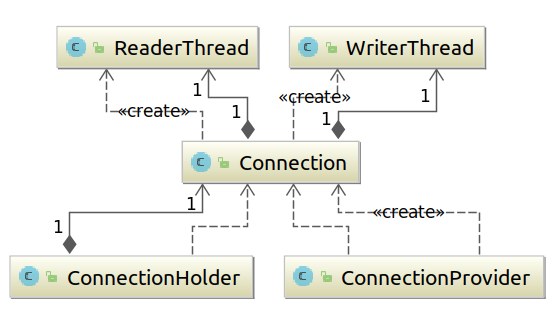
\includegraphics[width=0.6\linewidth]{img-net-d}
	\caption{Závislosti důležitých tříd.}
	\label{fig:img-net-d}
\end{figure}

\subsection{Ukázka práce se třídou Connection}
Následující příklad ukazuje práci se třídou Connection a zároveň způsob, jakým jsou realizovány integrační testy.
\begin{lstlisting}
@Test(timeout = DEFAULT_TIMEOUT)
public void testLogOut() throws Exception {
    try (Connection connection = ConnectionProvider.connect()) {

        Future<LogInResponse> inRes = connection.sendLogIn("Test");
        assertThat(inRes.get(), is(LogInResponse.OK));

        Future<LogOutResponse> outRes = connection.sendLogOut();
        assertThat(outRes.get(), is(LogOutResponse.OK));
    }
}
\end{lstlisting}


\newpage

\section{Protokol}
\paragraph{Formát}
Jedna zpráva se skládá z názvu instrukce a obsahu. Název instrukce má vždy 3 znaky. Od obsahu není ničím oddělen.

Jednotlivé zprávy jsou od sebe odděleny svislou čarou: \textbar.

\paragraph{Instrukce vysílané klientem}
\begin{itemize}
	\item \emph{BYE} -- vysílá klient nebo server, když se rozhodne ukončit spojení.
	Server jako poslední instrukci posílá také \emph{BYE}. 
	\item \emph{LIN {\textless}login{\textgreater}} -- přihlášení uživatele.\\
	Server odpovídá \emph{LIN {\textless}návratový kód{\textgreater}}. 
	\begin{itemize}
		\item OK = 0
		\item ALREADY\_LOGGED = 1
		\item NAME\_TOO\_SHORT = 2
		\item NAME\_TOO\_LONG = 3
		\item UNSUPPORTED\_CHARS = 4
		\item NAME\_ALREADY\_IN\_USE = 5
	\end{itemize}
	\item \emph{LOF} -- odhlášení uživatele.\\
	Server odpovídá \emph{LOF {\textless}návratový kód{\textgreater}}.
	\begin{itemize}
		\item OK = 0
		\item IN\_GAME = 1
	\end{itemize}
	\item \emph{GLI} -- požadavek na seznam her.\\
	Server odpovídá \emph{GLI {\textless}id${}_1${\textgreater},{\textless}výška${}_1${\textgreater},{\textless}šířka${}_1${\textgreater};{\textless}id${}_2${\textgreater}}\dots
	\item \emph{GPL {\textless}id{\textgreater}} -- požadavek na seznam hráčů ve hře.\\ 
	Server odpovídá \emph{GPL {\textless}jméno${}_1${\textgreater},{\textless}jméno${}_2${\textgreater}}\dots 
	\item \emph{GNW {\textless}šířka{\textgreater},{\textless}výška{\textgreater}} -- požadavek na vytvoření nové hry.\\
	Server odpovídá \emph{GNW {\textless}návratový kód{\textgreater}}.
	\begin{itemize}
		\item id nové hry \textgreater \space -1
		\item WRONG\_FORMAT = -1
		\item WRONG\_SIZE = -2
		\item NO\_PERMISSIONS = -3
	\end{itemize}
	\item \emph{GJO {\textless}id{\textgreater}} -- požadavek na připojení do hry.\\
	Server odpovídá \emph{GJO {\textless}návratový kód{\textgreater}}.
	\begin{itemize}
		\item OK = 0
		\item CANNOT\_JOIN = 1
		\item NO\_PERMISSIONS = 2
	\end{itemize}
	\item \emph{GST {\textless}id{\textgreater}} -- požadavek na herní stav určité hry.\\
	Server odpovídá seznamem dílků, po řádcích: \emph{GST {\textless}x${}_1${\textgreater},{\textless}y${}_1${\textgreater};{\textless}x${}_2${\textgreater}}\dots nebo \emph{GST error}
	\item \emph{GAC {\textless}id dílku${}_1${\textgreater},{\textless}x${}_1${\textgreater},{\textless}y${}_1${\textgreater};{\textless}id dílku${}_2${\textgreater}} -- herní akce.\\
	Server odpovídá \emph{GAC {\textless}návratový kód{\textgreater}}.
	\begin{itemize}
		\item OK = 0
		\item NO\_PERMISSIONS = 1
		\item WRONG\_FORMAT = 2
		\item WRONG\_PIECE = 3
	\end{itemize}
	\item \emph{GOF} -- odchod ze hry.
\end{itemize}

\paragraph{Instrukce vysílané serverem}
\begin{itemize}
	\item \emph{PIN} -- pro ověření spojení a validního klienta, vysílá server, klient odpovídá také \emph{PIN}.
	\item \emph{GUP {\textless}id dílku${}_1${\textgreater},{\textless}x${}_1${\textgreater},{\textless}y${}_1${\textgreater};{\textless}id dílku${}_2${\textgreater}} -- aktualizace herního stavu, seznam změněných dílků.
	\item \emph{GWI} -- rozesílá server hráčům při úspěšném dokončení hry.
\end{itemize}


\begin{figure}[H]
	\centering
	\begin{minipage}[b]{0.4\textwidth}
		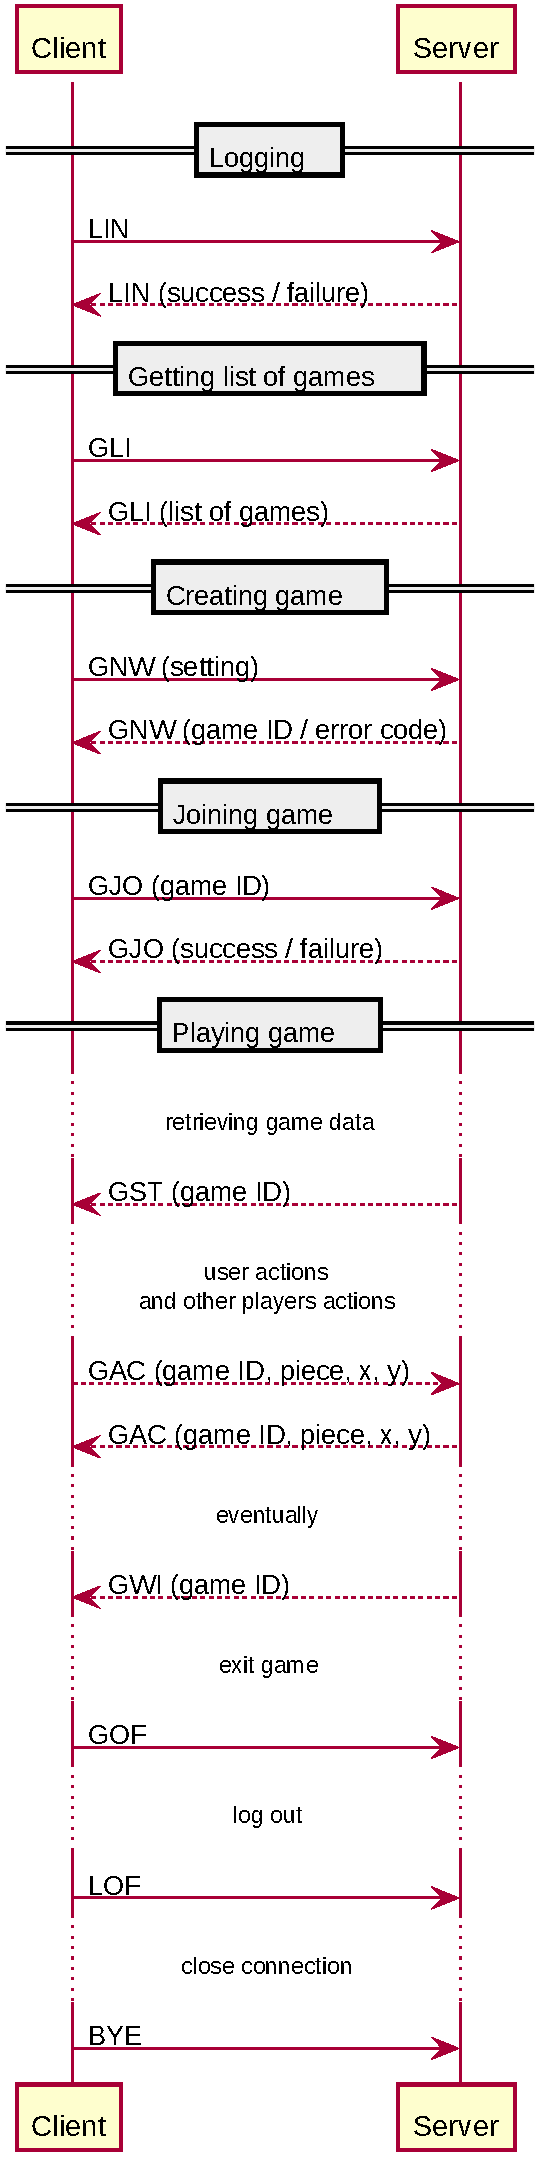
\includegraphics[width=0.85\linewidth]{sequence-diagram.pdf}
		\caption{Sekvenční diagram.}
		\label{fig:sequence-diagram.png}
	\end{minipage}
	\hfill
	\begin{minipage}[b]{0.4\textwidth}
		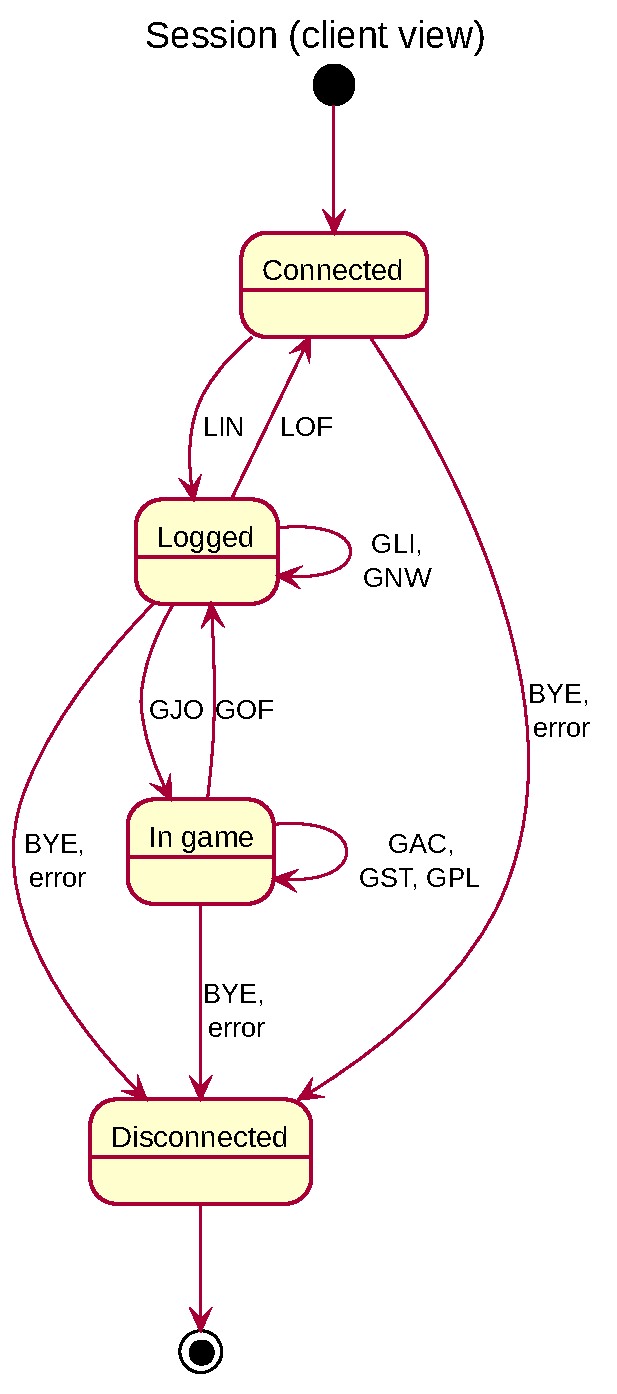
\includegraphics[width=0.9\linewidth]{state-diagram.pdf}
		\caption{Stavový diagram.}
		\label{fig:{state-diagram.png}}
	\end{minipage}
\end{figure}

\chapter{Uživatelská dokumentace}

\section{Pravidla hry}
Každý hráč má po přihlášení možnost připojit se ke hře nebo založit novou. Počet her je však omezen na 8. Po dokončení hry se jeden slot uvolní. Dokončení hry znamená složení dílků tak, aby do sebe zapadaly. K jedné hře se může připojit libovolný počet hráčů. Hráči se mohou v libovolnou chvíli odpojit i připojit.

\section{Server}

\paragraph{Sestavení}
Pro sestavení je vyžadován GNU Linux.
Sestavení proběhne po zadání příkazu \emph{make} v kořenovém adresáři serveru.

\paragraph{Spuštění}
Pro spuštění je vyžadován GNU Linux.
Spuštění proběhne po zadání příkazu \emph{./server-dist port}.
Pokud nebude port zadán, bude použit port s číslem 8076.

\paragraph{Ukončení}
Doporučený způsob ukončení je kombinací \emph{ctrl + c}.

\paragraph{Statistiky}
Při správném ukončení se statistiky uloží do souboru \emph{stats.txt} v aktuálním adresáři.

\paragraph{Logování}
Ve výchozím stavu je logování prováděno na standardní výstup. Pro logování do souboru musíme program spustit následovně: \emph{./server-dist port \textgreater log.txt}

\section{Klient}

\paragraph{Sestavení}
Pro sestavení je vyžadován nástroj JDK 8.
Sestavení proběhne po zadání \emph{gradlew} nebo \emph{gradlew.bat} do příkazové řádky v kořenovém adresáři klienta.

\paragraph{Spuštění}
Spuštění vyžaduje JRE 8. Program se spustí zadáním \emph{java -jar program.jar}.

\paragraph{Logování}
Ve výchozím stavu je logování chyb prováděno na standardní výstup a dále veškeré logování navíc do souboru \emph{log.txt}.

\begin{figure}[H]
	\centering
	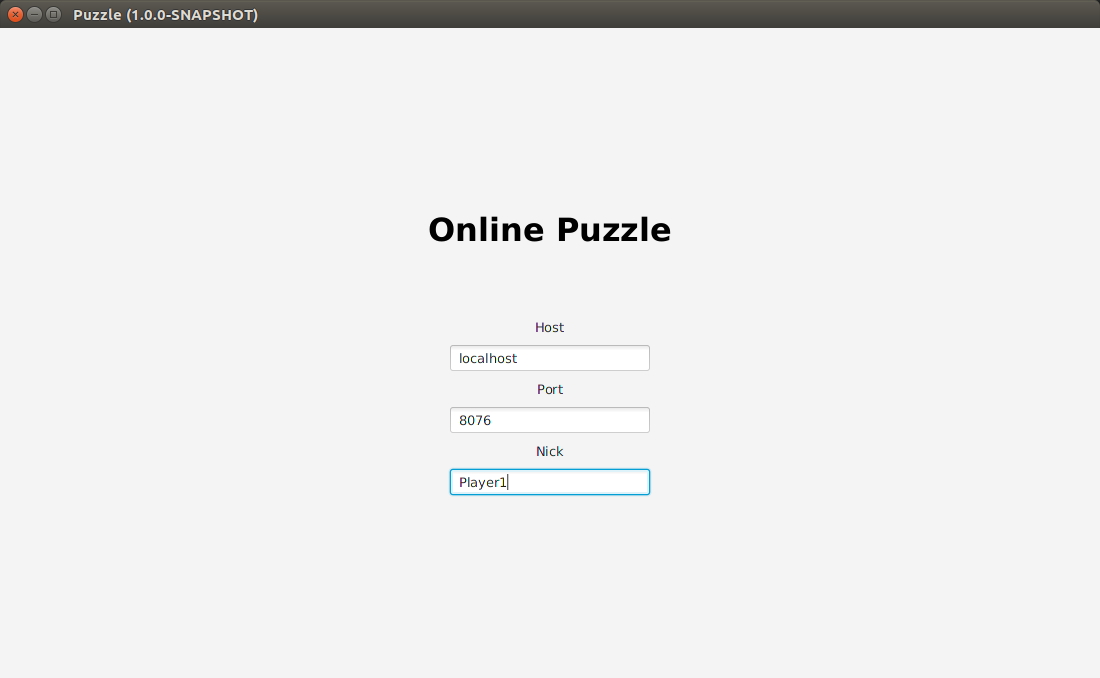
\includegraphics[width=1\linewidth]{img-scr-login}
	\caption{Stránka s přihlášením.}
\end{figure}

\begin{figure}[H]
	\centering
	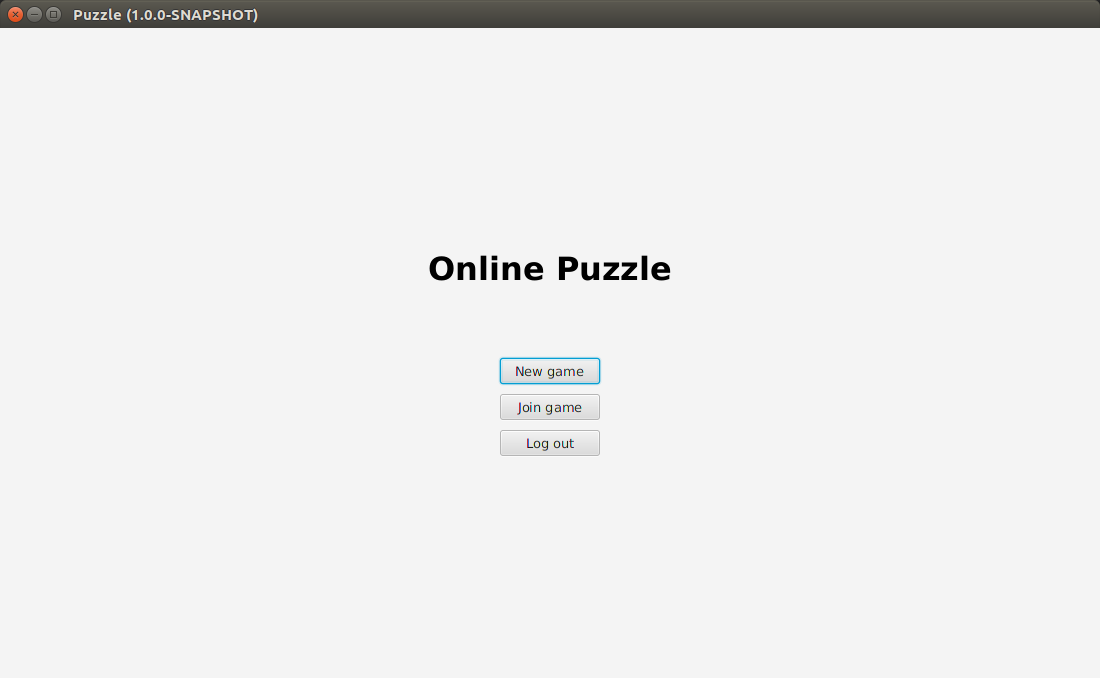
\includegraphics[width=1\linewidth]{img-scr-menu}
	\caption{Stránka s menu.}
\end{figure}

\begin{figure}[H]
	\centering
	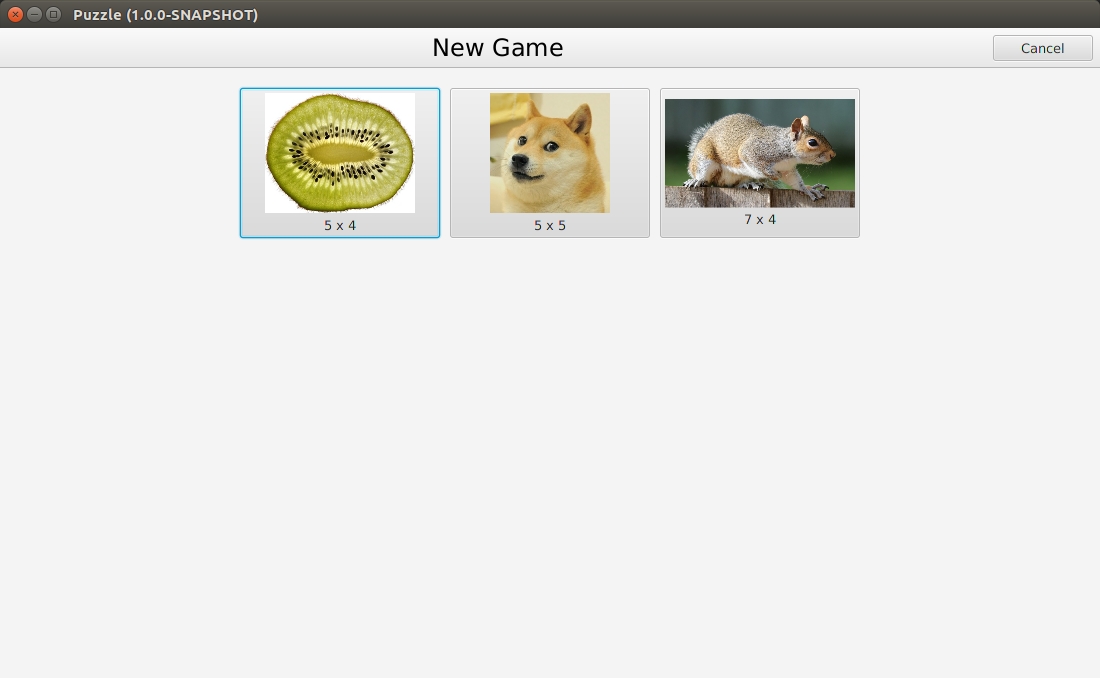
\includegraphics[width=1\linewidth]{img-scr-new}
	\caption{Stránka s vytvořením nové hry.}
\end{figure}

\begin{figure}[H]
	\centering
	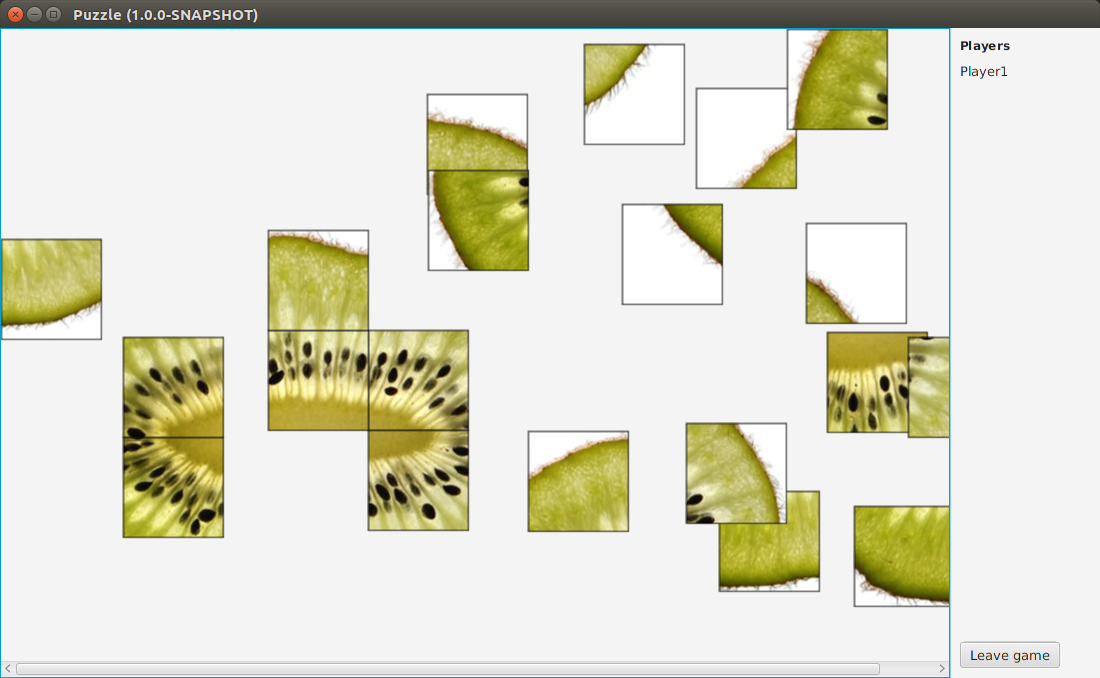
\includegraphics[width=1\linewidth]{img-scr-game}
	\caption{Stránka se hrou.}
\end{figure}

\end{document}